\documentclass[runningheads,orivec]{llncs} 
\usepackage{amsmath,amssymb,mathtools}
\usepackage{enumitem}
\usepackage{hyperref}
\usepackage{microtype}
\usepackage[T1]{fontenc}
\usepackage{booktabs}
% Figures (message-flow)
\usepackage{tikz}
\usetikzlibrary{calc,arrows.meta,positioning,calc}
\setlist[enumerate]{leftmargin=*,itemsep=0.25em}
% Algorithm boxes
\usepackage{algorithm}
\usepackage[noend]{algpseudocode}
\usepackage[section]{placeins}
\usepackage{float} % for H when absolutely needed
% dark PDF theme
\usepackage{xcolor}
\pagecolor[rgb]{0,0,0} %black
\color[rgb]{0.5,0.5,0.5} %grey

\newcommand{\prot}{\textsf{QuanTEEum}}
\newcommand{\sid}{\mathsf{sid}}
\newcommand{\Att}{\mathsf{AttestDelete}}
\newcommand{\RA}{\mathsf{RA}}
\newcommand{\FROST}{\textsf{FROST}}
\newcommand{\cFROST}{\FROST{}~\cite{komlo2020frost}}
\newcommand{\oss}{\textsf{OSS}}
\newcommand{\code}[1]{\texttt{#1}}

\begin{document}
\title{QuanTEEum: Quantum Cryptography via TEEs}
% \author{[Redacted for review]}
% \institute{[Redacted for review]}
\author{Shoaib Ahmed}
\institute{Cycles Protocol SA}
\maketitle

\begin{abstract}
One-shot signatures (OSS) have emerged as a versatile abstraction underpinning proposed blockchain applications including deterministic finality, quantum money, and ceremony-free SNARK parameters. Existing OSS constructions rely on quantum hardware that will not be widely available soon. Naïve emulations using a single trusted execution environment (TEE) inherit brittle unclonability requirements and concentrate integrity risk in one enclave. We present \prot{}, an honest-minority distributed protocol that realizes certified deletion and one-shot signing by running threshold signing entirely \emph{inside} independent TEEs. In \prot{}, $n$ enclaves run a threshold DKG, produce exactly one threshold signature on a designated statement, and each emits a remote-attestation (RA) binding an in-enclave deletion event. Security is \emph{additive}: every independent deletion attestation strictly raises the minimum attack cost, mitigating single-point TEE failures. We formalize certified deletion and one-shot signing in a remote-attestation model and show the attestation mechanism is pluggable: (a) conventional TEE RA, (b) cryptoeconomic attestations via escrowed collateral, and (c) future quantum instantiations, yielding a clean upgrade path. We sketch applications to single-shot block finality, quantum-money-flavored tokens, and de-facto ceremony-free CRS generation, and discuss liveness, freshness, and rollback subtleties.
\end{abstract}

\section{Introduction}
\paragraph{Motivation.}
OSS capture a powerful capability: make \emph{exactly-one} valid signature and then render any further signing infeasible. This single-use authenticity primitive cleanly abstracts (i) deterministic finality (each height signs once), (ii) quantum money (mint once, then unforgeable), and (iii) trusted-setup-free SNARK parameters (derive a CRS and then provably erase toxic waste). Yet today’s OSSs require quantum unclonability; TEEs offer a practical path but single-enclave designs reduce the guarantee to “trust this one box forever”.

\paragraph{Our approach.}
\prot{} lifts OSS to an \emph{honest-minority} setting by distributing the signing key across independent enclaves using a threshold DKG. The system produces one threshold signature on a frozen message and then aggregates per-enclave certified-deletion attestations bound to the session. The exact-one property reduces to the infeasibility of recovering a deleted threshold share from \emph{at least one} honest enclave, plus freshness/anti-replay for attestations.

\paragraph{Contributions.}
\begin{itemize}[leftmargin=*,itemsep=0.25em,topsep=0.25em]
  \item A formalization of certified deletion and one-shot signing in a remote-attestation model with explicit freshness and context binding.
  \item \prot{}: a threshold-in-TEE protocol that yields \emph{exactly one} threshold signature and a set of deletion attestations; security is additive across heterogeneous TEEs.
  \item A pluggable attestation mechanism: TEE RA today; cryptoeconomic attestations; future quantum erasure attestations---preserving the OSS API.
  \item Application sketches for (i) deterministic finality, (ii) quantum-money-style tokens, and (iii) de-facto ceremony-free CRS derivations.
  \item A discussion of liveness under abort, anti-replay, rollback resistance, and heterogeneity as defense-in-depth.
\end{itemize}

\section{Background and Model}
\subsection{One-shot signatures in brief}
An \oss{} scheme exposes $(\mathsf{Setup},\mathsf{KeyGen},\mathsf{SignOnce},\mathsf{Verify})$ with the property that for any keypair, at most one signature on at most one message is computationally feasible. Security is captured by a game where the adversary, after arbitrary queries \emph{except} a second signing, fails to produce two distinct valid signatures or one valid signature after certified deletion.

\subsection{Threshold signatures \cFROST{}}
We assume a Schnorr-style $t$-of-$n$ threshold signature with a secure DKG (e.g., \FROST{}). Parties hold additive shares $\{sk_i\}$ with public key $pk$, and interactive signing produces $\sigma$ on message $m$. Unforgeability holds if fewer than $t$ shares leak and nonces are not reused.

\subsection{TEE trust and remote attestation}
Each party $P_i$ hosts an enclave $E_i$ implementing \prot{}. We assume:
\begin{itemize}[leftmargin=*,itemsep=0.25em]
  \item \textbf{Code identity}: attestation binds a measurement (\emph{code hash}) and policy to outputs.
  \item \textbf{Sealed state semantics}: used only pre-signing to persist the DKG result across a crash.
  \item \textbf{Freshness/anti-replay}: a monotonic epoch is available (hardware counter or append-only log) and is bound into attestations.
  \item \textbf{Deletion API}: an enclave can make shares unrecoverable (\emph{zeroization}) and prove the transition with attestation carrying auxiliary data.
\end{itemize}
We \emph{do not} assume perfect side-channel resistance or that all rollback vectors are impossible; instead we bind acceptance to freshness predicates and a one-shot latch.

\subsection{Adversary and network}
The network is asynchronous with eventual delivery. The adversary may statically corrupt up to $f$ enclaves and their hosts and is rushing. We target $t=n$ for strongest one-shot semantics; extensions to $t<n$ are discussed in \S\ref{sec:discussion}.

\section{\prot{} Protocol}\label{sec:protocol}
\paragraph{Roles.} Parties $\{P_1,\dots,P_n\}$ run enclaves $\{E_1,\dots,E_n\}$. A (rotating) coordinator $C$ orchestrates rounds but learns no secrets.

\paragraph{Session binding.}
A session identifier $\mathsf{sid}$ is derived as
\[
  \mathsf{sid} \gets H(\mathsf{suite}\,\|\,\mathsf{policy}\,\|\,pk_{\mathrm{code}}\,\|\,m^{\star}\,\|\,\mathsf{nonce}).
\]

and is embedded in all protocol messages and in the attestation \emph{reportdata}. The designated message $m^{\star}$ is frozen by $C$ before signing.

\begin{figure}[!htbp]
\centering
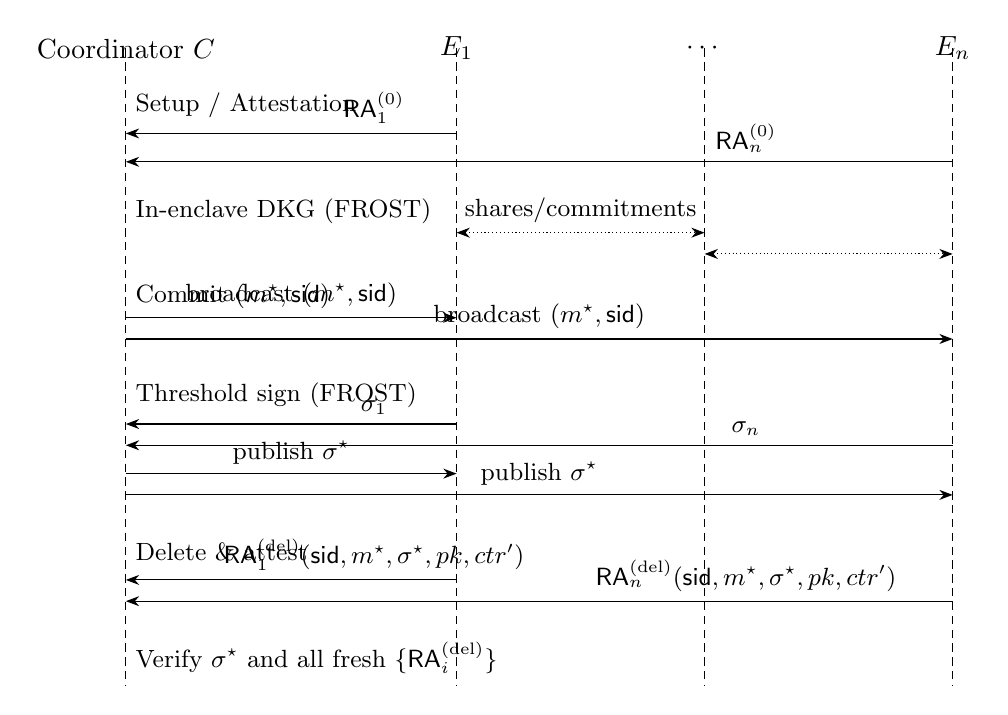
\begin{tikzpicture}[x=2.1cm,y=0.9cm,>=Stealth]
  % Columns / lifelines (labels at y=0)
  \node (C)  at (0,0)   {Coordinator $C$};
  \node (E1) at (2,0)   {$E_1$};
  \node (Ed) at (3.5,0) {$\cdots$};
  \node (En) at (5,0)   {$E_n$};

  % Lifeline verticals (dashed, starting under each label)
  \draw[densely dashed] ($(C)+(0,0)$)  -- +(0,-9);
  \draw[densely dashed] ($(E1)+(0,0)$) -- +(0,-9);
  \draw[densely dashed] ($(Ed)+(0,0)$) -- +(0,-9);
  \draw[densely dashed] ($(En)+(0,0)$) -- +(0,-9);

  % 1) Boot & initial quotes (arrows are horizontal: same y on both ends)
  \node[anchor=west] at ($(C)+(0,-0.8)$) {\small Setup / Attestation};
  \draw[->] ($(E1)+(0,-1.2)$) -- node[above,sloped,near start]{\small $\RA^{(0)}_1$} ($(C)+(0,-1.2)$);
  \draw[->] ($(En)+(0,-1.6)$) -- node[above,sloped,near start]{\small $\RA^{(0)}_n$} ($(C)+(0,-1.6)$);

  % 2) DKG (peer-to-peer, horizontal at fixed y's)
  \node[anchor=west] at ($(C)+(0,-2.3)$) {\small In-enclave DKG (FROST)};
  \draw[<->,densely dotted] ($(E1)+(0,-2.6)$) -- node[above]{\small shares/commitments} ($(Ed)+(0,-2.6)$);
  \draw[<->,densely dotted] ($(Ed)+(0,-2.9)$) -- ($(En)+(0,-2.9)$);

  % 3) Commit (freeze message / sid)
  \node[anchor=west] at ($(C)+(0,-3.5)$) {\small Commit $(m^{\star},\mathsf{sid})$};
  \draw[->] ($(C)+(0,-3.8)$) -- node[above,sloped]{\small broadcast $(m^{\star},\mathsf{sid})$} ($(E1)+(0,-3.8)$);
  \draw[->] ($(C)+(0,-4.1)$) -- node[above,sloped]{\small broadcast $(m^{\star},\mathsf{sid})$} ($(En)+(0,-4.1)$);

  % 4) Sign (partials to aggregate)
  \node[anchor=west] at ($(C)+(0,-4.9)$) {\small Threshold sign (FROST)};
  \draw[->] ($(E1)+(0,-5.3)$) -- node[above,sloped,near start]{\small $\sigma_1$} ($(C)+(0,-5.3)$);
  \draw[->] ($(En)+(0,-5.6)$) -- node[above,sloped,near start]{\small $\sigma_n$} ($(C)+(0,-5.6)$);
  \draw[->] ($(C)+(0,-6.0)$) -- node[above,sloped]{\small publish $\sigma^{\star}$} ($(E1)+(0,-6.0)$);
  \draw[->] ($(C)+(0,-6.3)$) -- node[above,sloped]{\small publish $\sigma^{\star}$} ($(En)+(0,-6.3)$);

  % 5) Certified deletion & quotes
  \node[anchor=west] at ($(C)+(0,-7.1)$) {\small Delete \& attest};
  \draw[->] ($(E1)+(0,-7.5)$) -- node[above,sloped,near start]{\small $\RA^{(\mathrm{del})}_1(\mathsf{sid},m^{\star},\sigma^{\star},pk,ctr')$} ($(C)+(0,-7.5)$);
  \draw[->] ($(En)+(0,-7.8)$) -- node[above,sloped,near start]{\small $\RA^{(\mathrm{del})}_n(\mathsf{sid},m^{\star},\sigma^{\star},pk,ctr')$} ($(C)+(0,-7.8)$);

  % 6) Acceptance (annotation only)
  \node[anchor=west] at ($(C)+(0,-8.6)$) {\small Verify $\sigma^{\star}$ and all fresh $\{\RA^{(\mathrm{del})}_i\}$};
\end{tikzpicture}
\caption{Protocol message flow for \prot{}: initial RA, in-enclave DKG, commit of $(m^{\star},\mathsf{sid})$, threshold signing, and post-delete attestations.}
\label{fig:flow}
\end{figure}

\subsection*{Interfaces and notation}
\begin{itemize}[leftmargin=*,itemsep=0.25em]
  \item \textsf{RA.GenQuote}$(\text{aux}) \to \RA$: produce a vendor-signed attestation over measurement and \code{aux}.
  \item \textsf{Fresh}$(\RA,\sid)$: predicate checking counter monotonicity and recency.
  \item \textsf{Del}(): irrecoverably zeroize in-enclave $sk_i$ and nonces.
\end{itemize}

\subsection{Setup and DKG}
\begin{enumerate}[leftmargin=*,itemsep=0.25em]
  \item Each $E_i$ boots, measures code, and publishes an initial quote $\RA_i^{(0)}$.
  \item Enclaves run a standard DKG inside enclaves to obtain additive shares $\{sk_i\}$ and public key $pk$; shares are held only in enclave memory, optionally sealed until signing starts.
\end{enumerate}

\begin{algorithm}[!htbp]
\caption{\prot{}: \emph{SetupAndDKG} (inside enclaves)}
\label{alg:setup}
\begin{small}
\begin{algorithmic}[1]
\State Each enclave $E_i$ boots; measure code $\mathsf{meas}$.
\State $\RA_i^{(0)} \gets \textsf{RA.GenQuote}(\text{aux} \gets \mathsf{meas})$; publish $\RA_i^{(0)}$.
\State All $E_i$ run in\mbox{-}enclave \FROST{} DKG $\to$ additive shares $sk_i$, public key $pk$.
\State Optionally \emph{seal} $sk_i$ until signing starts.
\State \textbf{return} $pk$ to the application (never $sk_i$).
\end{algorithmic}
\end{small}
\end{algorithm}

\subsection{Single-signing phase}
\begin{enumerate}
  \item \textbf{Commit.} $C$ chooses $m^{\star}$, derives $\mathsf{sid}$, broadcasts $(m^{\star},\mathsf{sid})$.
  \item \textbf{Latch.} Each $E_i$ verifies policy, binds $(m^{\star},\mathsf{sid})$ to its local one-shot latch, and bumps a monotonic epoch $ctr \leftarrow ctr{+}1$.
  \item \textbf{Sign.} Enclaves execute threshold signing (e.g., \FROST{}) on $m^{\star}$, producing partial signatures $\sigma_i$; $C$ aggregates to $\sigma^{\star}$.
\end{enumerate}

\begin{algorithm}[!htbp]
\caption{\prot{}: \emph{SingleSign} on designated message $m^{\star}$}
\label{alg:sign}
\begin{small}
\begin{algorithmic}[1]
\State Coordinator $C$ derives $\mathsf{sid} \gets H(\mathsf{suite}\,\|\,\mathsf{policy}\,\|\,\mathsf{meas}\,\|\,m^{\star}\,\|\,\mathsf{nonce})$.
\State $C$ broadcasts $(m^{\star},\mathsf{sid})$.
\For{each enclave $E_i$}
  \State Verify policy; bind $(m^{\star},\mathsf{sid})$ to one\mbox{-}shot latch; bump $ctr \leftarrow ctr{+}1$.
  \State Run \FROST{} partial signing on $m^{\star}$ to get $\sigma_i$; send to $C$.
\EndFor
\State $C$ aggregates $\{\sigma_i\}$ into $\sigma^{\star}$; publish $\sigma^{\star}$.
\State \textbf{return} $\sigma^{\star}$.
\end{algorithmic}
\end{small}
\end{algorithm}

\subsection{Certified deletion and verification}\label{sec:verify}
\begin{enumerate}
  \item \textbf{Delete \& attest.} Each $E_i$ executes \textsf{Del}(), records post-delete epoch $ctr'$, and generates $\RA_i^{(\mathrm{del})}$ over auxiliary data
  \[
    \textsf{aux}_i := (\mathsf{sid}\,\|\,m^{\star}\,\|\,\sigma^{\star}\,\|\,pk\,\|\,ctr').
  \]
  \item \textbf{Accept.} Verifier accepts iff (i) $\mathsf{Verify}(pk,m^{\star},\sigma^{\star})=1$, (ii) for a threshold $k$ (typically $k{=}n$), all $\{\RA_i^{(\mathrm{del})}\}$ validate under vendor roots and pass \textsf{Fresh}, and (iii) measurements and policy match the expected enclave code for \prot{}.
\end{enumerate}

\begin{algorithm}[!htbp]
\caption{\prot{}: \emph{DeleteAndVerify}}
\label{alg:delete-verify}
\begin{small}
\begin{algorithmic}[1]
\For{each enclave $E_i$}
  \State \textsf{Del}(): zeroize $sk_i$ and nonces; bump $ctr' \leftarrow ctr{+}1$.
  \State $\textsf{aux}_i \gets (\mathsf{sid}\,\|\,m^{\star}\,\|\,\sigma^{\star}\,\|\,pk\,\|\,ctr')$.
  \State $\RA_i^{(\mathrm{del})} \gets \textsf{RA.GenQuote}(\textsf{aux}_i)$; send to verifier.
\EndFor
\State \textbf{Accept} iff $\mathsf{Verify}(pk,m^{\star},\sigma^{\star})=1$ and at least $k$ quotes validate:
\State \hspace{1.2em}$\forall i\in Q:\ \textsf{VerifyRA}(\RA_i^{(\mathrm{del})})\wedge \textsf{Fresh}(\RA_i^{(\mathrm{del})},\mathsf{sid})\wedge \mathsf{meas}{=}\mathsf{expected}$.
\end{algorithmic}
\end{small}
\end{algorithm}

\subsection{Exact-one property}
The latch enforces a one-way state transition: any subsequent signing attempt with the same $\sid$ or with a new $\sid$ on the same enclave instance must verify $ctr$ strictly increases; \prot{} refuses pre-nonce sampling if either (a) \emph{post-delete} is set, or (b) the expected epoch monotonicity fails, preventing rollback-based nonce or key re-use.

\section{Security}\label{sec:security}
We sketch the core arguments; full proofs follow the standard game-hopping template with RA-oracle idealization.

\paragraph{Safety: one-shot unforgeability.}
\begin{theorem}[One-shot from threshold-in-TEE]\label{thm:one-shot}
Assume (i) the underlying threshold signature is unforgeable, (ii) at least one enclave is honest and transitions to post-delete state after producing $\sigma^{\star}$, (iii) \textsf{Fresh} prevents replay/rollback of pre-delete states, and (iv) vendor RA is unforgeable under the stated trust roots. Then producing two distinct valid signatures $(\sigma_1,\sigma_2)$ for the same $pk$ in session $\mathsf{sid}$ (on either same or distinct messages) is infeasible for PPT adversaries.
\end{theorem}

\begin{proof}[Proof sketch]
Suppose two signatures exist. If either is produced without $t$ valid shares, we break threshold unforgeability. Otherwise, at least $t$ shares were live at each signing. Because at least one honest enclave deleted its share and emitted $\RA^{(\mathrm{del})}$ bound to $(\mathsf{sid},m^{\star},\sigma^{\star})$, the only routes to a second signature are: (A) forge RA to claim deletion without deleting (contradicts RA unforgeability); (B) roll back the honest enclave to pre-delete (contradicts \textsf{Fresh}); (C) extract the honest enclave's share pre-delete (outside model unless SGX breaks); or (D) compromise enough enclaves across heterogeneous vendors (violates honest-minority).
\end{proof}

\paragraph{Liveness.}
With $t=n$ the protocol requires all enclaves to participate; a crashed or aborting enclave prevents progress. We adopt a bounded timeout: if signing fails, $C$ abandons $\sid$ and re-instantiates with fresh enclaves. In deployments desiring partial progress, \prot{} supports $t<n$ with two caveats: (i) erase attestations must reach $k\!\ge\!t$; (ii) the exact-one property is now conditioned on at least one of the $k$ attesting enclaves being honest.

\paragraph{Additive security via heterogeneity.}
If attestations are independent across vendors/geographies, the minimum attack cost is approximately the sum of per-enclave compromise costs (or, more conservatively, the minimum of all subsets of size $t$). We recommend explicit heterogeneity policies (e.g., “at least two vendors and three physical operators”).

\paragraph{Freshness and anti-replay.}
We require verifiers to check: (i) an enclave-specific monotonic counter $ctr'$ strictly increases across quotes, and (ii) the quote timestamp is recent, or (iii) an append-only public log includes the tuple $(\mathsf{sid},pk,m^{\star},\sigma^{\star},\mathsf{meas},ctr')$ before acceptance. Any quote with stale $ctr'$ or mismatched measurement is rejected.

\section{Applications}\label{sec:apps}
\subsection{Deterministic finality via one-shot chains}
For each height $h$, derive $\mathsf{sid}_h := H(h\,\|\,\textsf{policy}\,\|\,\cdots)$ and fix $m_h^{\star}$ to the block header. Validators (or a specialized \emph{finality committee}) host enclaves that run \prot{} to produce $\sigma_h^{\star}$ and deletion attestations. A block is \emph{final} when $(\sigma_h^{\star},\{\RA_i\})$ verifies. Safety reduces to Theorem~\ref{thm:one-shot}; liveness reduces to committee availability. Coordinator rotation prevents a single orchestrator from stalling progress.

\subsection{Quantum-money-flavored tokens}
Minting a token corresponds to running \prot{} with $m^{\star}$ encoding the serial and policy. Transfer can be modeled by \emph{re-minting} with a new serial bound to the recipient (or by embedding verification keys in a ledger that checks the one-shot predicate on spend). \prot{} supplies a classical OSS now; the same API can be “swapped” for quantum OSS later without redesign.

\subsection{De-facto ceremony-free CRS}
To derive a one-circuit CRS, set $m^{\star}$ to the transcript-to-be-signed, generate $\sigma^{\star}$, then erase all key material and nonces, attesting deletion. While this is not a plain-model proof of toxic-waste non-existence, it yields an auditable deletion trail with honest-minority robustness and heterogeneity, improving over single-operator ceremonies.

\section{Discussion and Future Work}\label{sec:discussion}
\paragraph{Why $t\!=\!n$ first?}
It maximizes the exact-one semantics and simplifies acceptance (\emph{all} attest). Generalizing to $t<n$ is straightforward mechanically but shifts the trust statement to “among the $k\!\ge\!t$ attesters, at least one honest enclave deleted.”

\paragraph{Nonce discipline.}
Nonce misuse is fatal in Schnorr. All nonce generation and aggregation must occur in-enclave; nonces are zeroized alongside shares and bound to $\sid$.

\paragraph{Rollback channels.}
Hardware monotonic counters are ideal but scarce; when unavailable, anchor \textsf{Fresh} in an append-only public log (e.g., consensus chain) and/or a replicated monotonicity oracle.

\paragraph{Cryptoeconomic attestations.}
Replace RA with bonded claims: each operator escrows collateral and signs a deletion statement $(\sid,m^{*},\sigma^{*})$ under a registered key; slashing conditions penalize equivocation or reuse. This yields weaker, but composable, guarantees and can be \emph{combined} with RA for stronger additivity.

\paragraph{Heterogeneity policy.}
Enforce at least two TEE vendors, distinct cloud providers, and distinct administrative domains. Acceptance SHOULD require a diversity predicate (e.g., vendor quorum).

\paragraph{Upgrade to quantum OSS.}
Once practical, swap the attestation mechanism for a quantum-certified deletion proof with the same acceptance predicate. Because \prot{} already binds $(\mathsf{sid},m^{\star},\sigma^{\star},pk)$ into attestations, the application layer remains unchanged.

\section{Conclusion}
\prot{} offers a deployable path to one-shot capabilities by composing threshold signatures with certified deletion inside heterogeneous TEEs. The exact-one property becomes an honest-minority statement with additive security across independent attestations. The same interface smoothly upgrades to future quantum OSS, enabling deterministic finality, quantum-money-like assets, and auditable substitutes for toxic-waste ceremonies.

\bibliographystyle{splncs04}
\bibliography{refs}
\end{document}